%%%%%%%%%%%%%%%%%%%%%%%%%%%%%%%%%%%%%%%%%
% University Assignment Title Page
% LaTeX Template
% Version 1.0 (27/12/12)
%
% This template has been downloaded from:
% http://www.LaTeXTemplates.com
%
% Original author:
% WikiBooks (http://en.wikibooks.org/wiki/LaTeX/Title_Creation)
%
% License:
% CC BY-NC-SA 3.0 (http://creativecommons.org/licenses/by-nc-sa/3.0/)
%
% Instructions for using this template:
% This title page is capable of being compiled as is. This is not useful for
% including it in another document. To do this, you have two options:
%
% 1) Copy/paste everything between \begin{document} and \end{document}
% starting at \begin{titlepage} and paste this into another LaTeX file where you
% want your title page.
% OR
% 2) Remove everything outside the \begin{titlepage} and \end{titlepage} and
% move this file to the same directory as the LaTeX file you wish to add it to.
% Then add %%%%%%%%%%%%%%%%%%%%%%%%%%%%%%%%%%%%%%%%%
% University Assignment Title Page
% LaTeX Template
% Version 1.0 (27/12/12)
%
% This template has been downloaded from:
% http://www.LaTeXTemplates.com
%
% Original author:
% WikiBooks (http://en.wikibooks.org/wiki/LaTeX/Title_Creation)
%
% License:
% CC BY-NC-SA 3.0 (http://creativecommons.org/licenses/by-nc-sa/3.0/)
%
% Instructions for using this template:
% This title page is capable of being compiled as is. This is not useful for
% including it in another document. To do this, you have two options:
%
% 1) Copy/paste everything between \begin{document} and \end{document}
% starting at \begin{titlepage} and paste this into another LaTeX file where you
% want your title page.
% OR
% 2) Remove everything outside the \begin{titlepage} and \end{titlepage} and
% move this file to the same directory as the LaTeX file you wish to add it to.
% Then add %%%%%%%%%%%%%%%%%%%%%%%%%%%%%%%%%%%%%%%%%
% University Assignment Title Page
% LaTeX Template
% Version 1.0 (27/12/12)
%
% This template has been downloaded from:
% http://www.LaTeXTemplates.com
%
% Original author:
% WikiBooks (http://en.wikibooks.org/wiki/LaTeX/Title_Creation)
%
% License:
% CC BY-NC-SA 3.0 (http://creativecommons.org/licenses/by-nc-sa/3.0/)
%
% Instructions for using this template:
% This title page is capable of being compiled as is. This is not useful for
% including it in another document. To do this, you have two options:
%
% 1) Copy/paste everything between \begin{document} and \end{document}
% starting at \begin{titlepage} and paste this into another LaTeX file where you
% want your title page.
% OR
% 2) Remove everything outside the \begin{titlepage} and \end{titlepage} and
% move this file to the same directory as the LaTeX file you wish to add it to.
% Then add %%%%%%%%%%%%%%%%%%%%%%%%%%%%%%%%%%%%%%%%%
% University Assignment Title Page
% LaTeX Template
% Version 1.0 (27/12/12)
%
% This template has been downloaded from:
% http://www.LaTeXTemplates.com
%
% Original author:
% WikiBooks (http://en.wikibooks.org/wiki/LaTeX/Title_Creation)
%
% License:
% CC BY-NC-SA 3.0 (http://creativecommons.org/licenses/by-nc-sa/3.0/)
%
% Instructions for using this template:
% This title page is capable of being compiled as is. This is not useful for
% including it in another document. To do this, you have two options:
%
% 1) Copy/paste everything between \begin{document} and \end{document}
% starting at \begin{titlepage} and paste this into another LaTeX file where you
% want your title page.
% OR
% 2) Remove everything outside the \begin{titlepage} and \end{titlepage} and
% move this file to the same directory as the LaTeX file you wish to add it to.
% Then add \input{./title_page_1.tex} to your LaTeX file where you want your
% title page.
%
%%%%%%%%%%%%%%%%%%%%%%%%%%%%%%%%%%%%%%%%%

%----------------------------------------------------------------------------------------
%	PACKAGES AND OTHER DOCUMENT CONFIGURATIONS
%----------------------------------------------------------------------------------------

\documentclass[12pt]{article}
\usepackage[utf8]{inputenc}
\usepackage{epigraph}
\usepackage{setspace}
\usepackage[textwidth=3cm, shadow]{todonotes}
\usepackage{mdwlist}
\usepackage{hyperref}

\onehalfspacing
\begin{document}


\begin{titlepage}

\newcommand{\HRule}{\rule{\linewidth}{0.5mm}} % Defines a new command for the 
%horizontal lines, change thickness here

\center % Center everything on the page

%----------------------------------------------------------------------------------------
%	HEADING SECTIONS
%----------------------------------------------------------------------------------------

\textsc{\LARGE Universität Leipzig}\\[1.5cm] % Name of your university/college
\textsc{\Large Hausarbeit}\\[0.5cm] % Major heading such as course name
\textsc{\large zum Seminarvortrag "Free Software Foundation Europe"}\\[0.5cm] % 
% Minor heading such as course title

%----------------------------------------------------------------------------------------
%	TITLE SECTION
%----------------------------------------------------------------------------------------

\HRule \\[0.4cm]
{ \LARGE \bfseries Free Software Foundation Europe und Lobbying}\\[0.4cm]
%Title of your document
\HRule \\[1.5cm]

%----------------------------------------------------------------------------------------
%	AUTHOR SECTION
%----------------------------------------------------------------------------------------

\begin{minipage}{0.4\textwidth}
\begin{flushleft} \large
\emph{Author:}\\
Sascha \textsc{Ebert} % Your name
\end{flushleft}
\end{minipage}
~
\begin{minipage}{0.4\textwidth}
\begin{flushright} \large
\emph{Supervisor:} \\
Prof. Dr. H.-G. \textsc{Gräbe} % Supervisor's Name
\end{flushright}
\end{minipage}\\[4cm]

% If you don't want a supervisor, uncomment the two lines below and remove the 
%section above
%\Large \emph{Author:}\\
%John \textsc{Smith}\\[3cm] % Your name

%----------------------------------------------------------------------------------------
%	DATE SECTION
%----------------------------------------------------------------------------------------

{\large \today}\\[3cm] % Date, change the \today to a set date if you want to 
% be 
% precise
\newpage
''Sharing is good, and with digital technology, sharing is easy.``

Richard Stallman



%----------------------------------------------------------------------------------------
%	LOGO SECTION
%----------------------------------------------------------------------------------------

%\includegraphics{Logo}\\[1cm] % Include a department/university logo - this 
% will require the graphicx package

%----------------------------------------------------------------------------------------

\vfill % Fill the rest of the page with whitespace

\end{titlepage}

\tableofcontents
\newpage

\section{Einleitung}
\epigraph{We believe in cooperation and transparency.}{FSFE}
Die öffentlichen Worte der Free Software Foundation Europe (FSFE) sind deutlich. 
Es geht
um das Verwirklichen ihrer Kernziele mit Hilfe eines transparenten 
Aktionsmusters.
Dieses Statement überrascht kaum, da sich die FSFE die Erhaltung der Vision von 
``Free Software'' zum Ziel gemacht hat, dessen Definition gerade die Gedanken 
``Transparenz'' und ``Korporation'' als absolute Kernfaktoren enthält. Es ergibt 
sich somit direkt folgend die Forderung, die Folgen der Definition des Begriffes 
"Free Software" konsistent in ihre Struktur und Organisation zu übertragen.

Die Frage der Finanzierung der FSFE und deren Arbeit in diversen
Kampagnen bildet nun das Gerüst für einen intuitiven Lobbyismusvorwurf. Dieser 
muss klar ausgeführt werden und mit Hilfe
verschiedener Werke auf die ausgiebige Reichweite und Komplexität
des Begriffs angewendet werden.

Diese Arbeit schickt sich an die Gestalt und Struktur der Free Software 
Foundation Europe zu erläutern, den eben genannten Vorwurf zu spezifizieren und 
theoretisch zu behandeln inwiefern und in welchen Formen die FSFE Lobbying 
betreibt. Ergänzend soll ein Vergleich gegenüber anderen Lobbyismusstrukturen,
wie die der Pharmaindustrie geführt werden, um auf die spezielle Verbindung 
zwischen dem Thema der FSFE und dem Lobbyismus aufmerksam zu machen.
\newpage

\section{Free Software Foundation Europe}
\epigraph{Free Software Foundation Europe is a charity that empowers
users to control technology.}{FSFE}
Seit ihrer Gründung am 10. März 2001 hat die FSFE einen Langen Weg der 
Vertretung Freier Software bestritten. Es handelt sich bei der FSFE 
um eine gemeinnützige regierungsunabhängige Organisation (NGO), welche sich
auf der deutschen Rechtsform des e.V. gründet. Nach Georg 
Greve und Karsten Gerloff ist Matthias Kirschner nunmehr der bereits 3. 
Präsident der FSFE. Schon der Gründer George Greves formulierte die Ziele der 
FSFE sehr deutlich indem er verschiedene Bedrohungen für Freie Software 
erkannte und die FSFE als Institution - um diesen Bedrohungen gegenüber zu 
stehen - ins Leben rief.\cite{PLGreveInterView} \todo{Mehr Bedrohungen 
erläutern}Er führt Softwarepatente und Richtlinien wie z.B. die EUCD, IPRED und 
\todo{Richtlinien anschauen}WIPO als Beispiele für diese Gefahren auf.

\subsection{Freie Software}
Diesem Bestreben liegt natürlich eine klar definierte Auffassung des Terminus 
"Freie Software" zu Grunde. Dabei legt die FSFE folgende vier
Rechte gegenüber der Nutzung von Freier Software zu Grunde. Zum Einen
wird die Freiheit eingeräumt, ein Programm für alle erdenklichen Zwecke zu 
nutzen, was z.B. die Einschränkung von Nutzungsräumen verbietet oder
auch sogar konträr dagegen die Nutzung der Software im kommerziellen Rahmen 
durchaus
erlaubt. Weiterhin muss es möglich sein die Struktur und Funktionsweise des 
Programms studieren und sie entsprechend
anpassen zu können, was die Notwendigkeit für das Offenlegen des Quellcodes 
liefert. Außerdem wird argumentiert, dass es möglich ist, Software mit einem 
nahzu gegen Null gehenden Aufwand zu kopieren, woraus das Recht abgeleitet wird
die Software weiter geben zu dürfen. Den
vierten und letzten Pfeiler stellt die Freiheit, des betrachtete Programm
jederzeit verbessern beziehungsweise verändern zu können, wobei auch eine 
Veröffentlichung dieser Änderung möglich sein muss.\cite{FsfeFs}

Freie Software wird oft in Assoziation zu Open Source Software gesetzt. Die
FSFE weißt hier eindrücklich darauf hin, dass dieser Begriff bereits aufgeweicht
ist und auch Produkte damit bezeichnet werden, welche z.B nur sehr beschränkten
Zugriff zu Teilen des Quellcodes zulassen.

\subsection{Aufbau des Vereins}
Um nun die Handlungsgrundlagen der FSFE weiter zu verstehen, ist es nötig
die Struktur der Organisation zu analysieren, da die Hierarchie den 
Entscheidungsprozess natürlicherweise beeinflusst. \todo{Schluss: fehlende 
Transparenz ohne persönliche Beziehungen}Wie bereits erwähnt handelt es sich bei
der FSFE um einen gemeinnützigen Verein welcher einen Vereinsvorsitzenden 
(Präsident) benötigt. Dieses Amt hat gerade Matthias Kirschner inne, welcher im 
Gegensatz zu George Greve einen eher nicht technischen Hintergrund aufweist.
Kirschner's Hauptziel ist eindeutig die Kontrollmöglichkeit von Technologie 
durch ihre Nutzer. Als Weg dahin sieht er unter anderem die Aufklärungsarbeit 
der FSFE durch Werbekampagnen und individuelle
Beratung.\cite{TAZKirschnerInterView} \cite{YTKirschnerInterView}

Kirschner ist einer von derzeit 8 Vollzeitangestellten.\cite{FsfeTeam} Den
Rest des Vereins bilden ehrenamtliche Mitarbeiter,\todo{Themenbreiche 
erläutern} welche alle feste 
Themenbereiche besitzen. Viele \todo{fraglich} 
der gelisteten Mitglieder weißen 
einen 
Hintergrund auf in welchem sie schon mit zu Freier Software äquivalenten Themen 
in Berührung gekommen sind. So war Jonas Öberg zum Beispiel Fellow für die
Shuttleworth Foundation. Weiterhin gibt es auch Mitbeteiligte wie Fernanda 
Weiden, welche in Firmen wie Facebook arbeiten.\cite{FsfeTeam}

Nach Aussagen von George Greve reicht gerade die Anzahl der voll bezahlten 
Mitglieder nicht aus, um genügend politische Arbeit auf Landesebene zu 
betreiben. Hier sollte es für jedes Land mindestens eine voll honorierte Person
geben was aber zumindest im Jahr 2004 noch das Budget 
sprengte.\cite{PLGreveInterView}

Greve, Kirschner und Öberg sind Teil des Exekutivrates, welcher prinzipiell
die alleinige Entscheidungsgewalt besitzt. Greve mahnte hier allerdings an, dass
es einen grundsätzlich demokratischen Entscheidungsfindungsprozess gibt und 
noch nie jemand aus diesem ausgeschlossen wurde.

\subsubsection{Fellowships}
Ein weiteres Standbein der FSFE bildet das Fellowship-Programm womit
grundsätzlich Jedem ermöglicht wird innerhalb der FSFE Einfluss zu nehmen.
Voraussetzung hierfür ist - wie in einem gemeinnützigen Verein üblich - das 
Entrichten eines Mitgliedsbeitrags, der variabel
wählbar ist. Hierdurch ist es möglich entweder reines Fördermitglied zu werden
oder, durch die Mitgliedschaft berechtigt, Zugang zu den FSFE-internen Systemen 
und Arbeiten anderer Fellowship-Teilnehmer zu bekommen, oder eine lokale Gruppe
zu gründen welche die FSFE vertritt. Der allgemeine Nutzen des 
Fellowship-Programmes bestehen für die FSFE darin, das Thema ''Freie Software`` 
in 
den Köpfen auch der Menschen zu halten, welche nicht auf täglicher Basis mit 
diesem Gebiet direkt konfrontiert werden. Dabei wird aber darauf hingewiesen, 
das sehr wohl viele Leute Freie Software ohne das Bewusstsein darüber einsetzen.


\todo[inline]{Über Lizenzthematik nachdenken}

\section{Lobbyismusbegriff}
\subsection{Begriff}
\begin{itemize*}
    \item Begriff erläutern durch \cite{LeifSpeth200312}
    \item Anatomie erläutern
\end{itemize*}

\section{Die FSFE als Lobbyorganisation}
\begin{itemize*}
    \item Lobbydef aufFSFE  anwenden und dabei FSFE Weiter erklären
    \item Aussagen von Greve Benutzen \cite{PLGreveInterView}
\end{itemize*}

\subsection{Wirken der FSFE - Kampagnen}
Die Arbeit der FSFE findet unter anderem in unterschiedlichen Kampagnen statt, 
welche die Grundlage für die meinungsbildende Wirkung der Organisation stellt.
\begin{itemize*}
    \item Secureboot anschauen -- Einflusssicherungsversuch von anderen
    Unternehmen
\end{itemize*}

\begin{itemize*}
\item Finanzierung I
\item Finanzierung II
\item welcher Einfluss ergibt sich dadurch
\item welche Unternehmen haben wie Einfluss auf die FSFE?
\end{itemize*}

\section{Unterschied zu anderen Lobbyingarten}
\begin{itemize*}
\item Pharmalobby \cite{BeckLobbyGesundwe}
\item Agrar-Lobbying
\item IT-Lobby
\item struktureller Vergleich
\item finanzieller Vergleich
\item regionaler Vergleich (Weltweit, Europa, Landesebene)
\item Transparenz, Transparenz, Transparenz!!!
\end{itemize*}

\section{Schluss}
\begin{itemize*}
\item Lobbying als natürlicher Vorgang (Eigene These)
\item Klare Unterschiede Intensität
\end{itemize*}

\newpage
\bibliography{refs}
\bibliographystyle{IEEEtran}
\todo[inline]{Bibtexvorlage der Uni benutzen}
\todo[inline]{Unterlagen zuhause checken}

\listoftodos

\end{document}
 to your LaTeX file where you want your
% title page.
%
%%%%%%%%%%%%%%%%%%%%%%%%%%%%%%%%%%%%%%%%%

%----------------------------------------------------------------------------------------
%	PACKAGES AND OTHER DOCUMENT CONFIGURATIONS
%----------------------------------------------------------------------------------------

\documentclass[12pt]{article}
\usepackage[utf8]{inputenc}
\usepackage{epigraph}
\usepackage{setspace}
\usepackage[textwidth=3cm, shadow]{todonotes}
\usepackage{mdwlist}
\usepackage{hyperref}

\onehalfspacing
\begin{document}


\begin{titlepage}

\newcommand{\HRule}{\rule{\linewidth}{0.5mm}} % Defines a new command for the 
%horizontal lines, change thickness here

\center % Center everything on the page

%----------------------------------------------------------------------------------------
%	HEADING SECTIONS
%----------------------------------------------------------------------------------------

\textsc{\LARGE Universität Leipzig}\\[1.5cm] % Name of your university/college
\textsc{\Large Hausarbeit}\\[0.5cm] % Major heading such as course name
\textsc{\large zum Seminarvortrag "Free Software Foundation Europe"}\\[0.5cm] % 
% Minor heading such as course title

%----------------------------------------------------------------------------------------
%	TITLE SECTION
%----------------------------------------------------------------------------------------

\HRule \\[0.4cm]
{ \LARGE \bfseries Free Software Foundation Europe und Lobbying}\\[0.4cm]
%Title of your document
\HRule \\[1.5cm]

%----------------------------------------------------------------------------------------
%	AUTHOR SECTION
%----------------------------------------------------------------------------------------

\begin{minipage}{0.4\textwidth}
\begin{flushleft} \large
\emph{Author:}\\
Sascha \textsc{Ebert} % Your name
\end{flushleft}
\end{minipage}
~
\begin{minipage}{0.4\textwidth}
\begin{flushright} \large
\emph{Supervisor:} \\
Prof. Dr. H.-G. \textsc{Gräbe} % Supervisor's Name
\end{flushright}
\end{minipage}\\[4cm]

% If you don't want a supervisor, uncomment the two lines below and remove the 
%section above
%\Large \emph{Author:}\\
%John \textsc{Smith}\\[3cm] % Your name

%----------------------------------------------------------------------------------------
%	DATE SECTION
%----------------------------------------------------------------------------------------

{\large \today}\\[3cm] % Date, change the \today to a set date if you want to 
% be 
% precise
\newpage
''Sharing is good, and with digital technology, sharing is easy.``

Richard Stallman



%----------------------------------------------------------------------------------------
%	LOGO SECTION
%----------------------------------------------------------------------------------------

%\includegraphics{Logo}\\[1cm] % Include a department/university logo - this 
% will require the graphicx package

%----------------------------------------------------------------------------------------

\vfill % Fill the rest of the page with whitespace

\end{titlepage}

\tableofcontents
\newpage

\section{Einleitung}
\epigraph{We believe in cooperation and transparency.}{FSFE}
Die öffentlichen Worte der Free Software Foundation Europe (FSFE) sind deutlich. 
Es geht
um das Verwirklichen ihrer Kernziele mit Hilfe eines transparenten 
Aktionsmusters.
Dieses Statement überrascht kaum, da sich die FSFE die Erhaltung der Vision von 
``Free Software'' zum Ziel gemacht hat, dessen Definition gerade die Gedanken 
``Transparenz'' und ``Korporation'' als absolute Kernfaktoren enthält. Es ergibt 
sich somit direkt folgend die Forderung, die Folgen der Definition des Begriffes 
"Free Software" konsistent in ihre Struktur und Organisation zu übertragen.

Die Frage der Finanzierung der FSFE und deren Arbeit in diversen
Kampagnen bildet nun das Gerüst für einen intuitiven Lobbyismusvorwurf. Dieser 
muss klar ausgeführt werden und mit Hilfe
verschiedener Werke auf die ausgiebige Reichweite und Komplexität
des Begriffs angewendet werden.

Diese Arbeit schickt sich an die Gestalt und Struktur der Free Software 
Foundation Europe zu erläutern, den eben genannten Vorwurf zu spezifizieren und 
theoretisch zu behandeln inwiefern und in welchen Formen die FSFE Lobbying 
betreibt. Ergänzend soll ein Vergleich gegenüber anderen Lobbyismusstrukturen,
wie die der Pharmaindustrie geführt werden, um auf die spezielle Verbindung 
zwischen dem Thema der FSFE und dem Lobbyismus aufmerksam zu machen.
\newpage

\section{Free Software Foundation Europe}
\epigraph{Free Software Foundation Europe is a charity that empowers
users to control technology.}{FSFE}
Seit ihrer Gründung am 10. März 2001 hat die FSFE einen Langen Weg der 
Vertretung Freier Software bestritten. Es handelt sich bei der FSFE 
um eine gemeinnützige regierungsunabhängige Organisation (NGO), welche sich
auf der deutschen Rechtsform des e.V. gründet. Nach Georg 
Greve und Karsten Gerloff ist Matthias Kirschner nunmehr der bereits 3. 
Präsident der FSFE. Schon der Gründer George Greves formulierte die Ziele der 
FSFE sehr deutlich indem er verschiedene Bedrohungen für Freie Software 
erkannte und die FSFE als Institution - um diesen Bedrohungen gegenüber zu 
stehen - ins Leben rief.\cite{PLGreveInterView} \todo{Mehr Bedrohungen 
erläutern}Er führt Softwarepatente und Richtlinien wie z.B. die EUCD, IPRED und 
\todo{Richtlinien anschauen}WIPO als Beispiele für diese Gefahren auf.

\subsection{Freie Software}
Diesem Bestreben liegt natürlich eine klar definierte Auffassung des Terminus 
"Freie Software" zu Grunde. Dabei legt die FSFE folgende vier
Rechte gegenüber der Nutzung von Freier Software zu Grunde. Zum Einen
wird die Freiheit eingeräumt, ein Programm für alle erdenklichen Zwecke zu 
nutzen, was z.B. die Einschränkung von Nutzungsräumen verbietet oder
auch sogar konträr dagegen die Nutzung der Software im kommerziellen Rahmen 
durchaus
erlaubt. Weiterhin muss es möglich sein die Struktur und Funktionsweise des 
Programms studieren und sie entsprechend
anpassen zu können, was die Notwendigkeit für das Offenlegen des Quellcodes 
liefert. Außerdem wird argumentiert, dass es möglich ist, Software mit einem 
nahzu gegen Null gehenden Aufwand zu kopieren, woraus das Recht abgeleitet wird
die Software weiter geben zu dürfen. Den
vierten und letzten Pfeiler stellt die Freiheit, des betrachtete Programm
jederzeit verbessern beziehungsweise verändern zu können, wobei auch eine 
Veröffentlichung dieser Änderung möglich sein muss.\cite{FsfeFs}

Freie Software wird oft in Assoziation zu Open Source Software gesetzt. Die
FSFE weißt hier eindrücklich darauf hin, dass dieser Begriff bereits aufgeweicht
ist und auch Produkte damit bezeichnet werden, welche z.B nur sehr beschränkten
Zugriff zu Teilen des Quellcodes zulassen.

\subsection{Aufbau des Vereins}
Um nun die Handlungsgrundlagen der FSFE weiter zu verstehen, ist es nötig
die Struktur der Organisation zu analysieren, da die Hierarchie den 
Entscheidungsprozess natürlicherweise beeinflusst. \todo{Schluss: fehlende 
Transparenz ohne persönliche Beziehungen}Wie bereits erwähnt handelt es sich bei
der FSFE um einen gemeinnützigen Verein welcher einen Vereinsvorsitzenden 
(Präsident) benötigt. Dieses Amt hat gerade Matthias Kirschner inne, welcher im 
Gegensatz zu George Greve einen eher nicht technischen Hintergrund aufweist.
Kirschner's Hauptziel ist eindeutig die Kontrollmöglichkeit von Technologie 
durch ihre Nutzer. Als Weg dahin sieht er unter anderem die Aufklärungsarbeit 
der FSFE durch Werbekampagnen und individuelle
Beratung.\cite{TAZKirschnerInterView} \cite{YTKirschnerInterView}

Kirschner ist einer von derzeit 8 Vollzeitangestellten.\cite{FsfeTeam} Den
Rest des Vereins bilden ehrenamtliche Mitarbeiter,\todo{Themenbreiche 
erläutern} welche alle feste 
Themenbereiche besitzen. Viele \todo{fraglich} 
der gelisteten Mitglieder weißen 
einen 
Hintergrund auf in welchem sie schon mit zu Freier Software äquivalenten Themen 
in Berührung gekommen sind. So war Jonas Öberg zum Beispiel Fellow für die
Shuttleworth Foundation. Weiterhin gibt es auch Mitbeteiligte wie Fernanda 
Weiden, welche in Firmen wie Facebook arbeiten.\cite{FsfeTeam}

Nach Aussagen von George Greve reicht gerade die Anzahl der voll bezahlten 
Mitglieder nicht aus, um genügend politische Arbeit auf Landesebene zu 
betreiben. Hier sollte es für jedes Land mindestens eine voll honorierte Person
geben was aber zumindest im Jahr 2004 noch das Budget 
sprengte.\cite{PLGreveInterView}

Greve, Kirschner und Öberg sind Teil des Exekutivrates, welcher prinzipiell
die alleinige Entscheidungsgewalt besitzt. Greve mahnte hier allerdings an, dass
es einen grundsätzlich demokratischen Entscheidungsfindungsprozess gibt und 
noch nie jemand aus diesem ausgeschlossen wurde.

\subsubsection{Fellowships}
Ein weiteres Standbein der FSFE bildet das Fellowship-Programm womit
grundsätzlich Jedem ermöglicht wird innerhalb der FSFE Einfluss zu nehmen.
Voraussetzung hierfür ist - wie in einem gemeinnützigen Verein üblich - das 
Entrichten eines Mitgliedsbeitrags, der variabel
wählbar ist. Hierdurch ist es möglich entweder reines Fördermitglied zu werden
oder, durch die Mitgliedschaft berechtigt, Zugang zu den FSFE-internen Systemen 
und Arbeiten anderer Fellowship-Teilnehmer zu bekommen, oder eine lokale Gruppe
zu gründen welche die FSFE vertritt. Der allgemeine Nutzen des 
Fellowship-Programmes bestehen für die FSFE darin, das Thema ''Freie Software`` 
in 
den Köpfen auch der Menschen zu halten, welche nicht auf täglicher Basis mit 
diesem Gebiet direkt konfrontiert werden. Dabei wird aber darauf hingewiesen, 
das sehr wohl viele Leute Freie Software ohne das Bewusstsein darüber einsetzen.


\todo[inline]{Über Lizenzthematik nachdenken}

\section{Lobbyismusbegriff}
\subsection{Begriff}
\begin{itemize*}
    \item Begriff erläutern durch \cite{LeifSpeth200312}
    \item Anatomie erläutern
\end{itemize*}

\section{Die FSFE als Lobbyorganisation}
\begin{itemize*}
    \item Lobbydef aufFSFE  anwenden und dabei FSFE Weiter erklären
    \item Aussagen von Greve Benutzen \cite{PLGreveInterView}
\end{itemize*}

\subsection{Wirken der FSFE - Kampagnen}
Die Arbeit der FSFE findet unter anderem in unterschiedlichen Kampagnen statt, 
welche die Grundlage für die meinungsbildende Wirkung der Organisation stellt.
\begin{itemize*}
    \item Secureboot anschauen -- Einflusssicherungsversuch von anderen
    Unternehmen
\end{itemize*}

\begin{itemize*}
\item Finanzierung I
\item Finanzierung II
\item welcher Einfluss ergibt sich dadurch
\item welche Unternehmen haben wie Einfluss auf die FSFE?
\end{itemize*}

\section{Unterschied zu anderen Lobbyingarten}
\begin{itemize*}
\item Pharmalobby \cite{BeckLobbyGesundwe}
\item Agrar-Lobbying
\item IT-Lobby
\item struktureller Vergleich
\item finanzieller Vergleich
\item regionaler Vergleich (Weltweit, Europa, Landesebene)
\item Transparenz, Transparenz, Transparenz!!!
\end{itemize*}

\section{Schluss}
\begin{itemize*}
\item Lobbying als natürlicher Vorgang (Eigene These)
\item Klare Unterschiede Intensität
\end{itemize*}

\newpage
\bibliography{refs}
\bibliographystyle{IEEEtran}
\todo[inline]{Bibtexvorlage der Uni benutzen}
\todo[inline]{Unterlagen zuhause checken}

\listoftodos

\end{document}
 to your LaTeX file where you want your
% title page.
%
%%%%%%%%%%%%%%%%%%%%%%%%%%%%%%%%%%%%%%%%%

%----------------------------------------------------------------------------------------
%	PACKAGES AND OTHER DOCUMENT CONFIGURATIONS
%----------------------------------------------------------------------------------------

\documentclass[12pt]{article}
\usepackage[utf8]{inputenc}
\usepackage{epigraph}
\usepackage{setspace}
\usepackage[textwidth=3cm, shadow]{todonotes}
\usepackage{mdwlist}
\usepackage{hyperref}

\onehalfspacing
\begin{document}


\begin{titlepage}

\newcommand{\HRule}{\rule{\linewidth}{0.5mm}} % Defines a new command for the 
%horizontal lines, change thickness here

\center % Center everything on the page

%----------------------------------------------------------------------------------------
%	HEADING SECTIONS
%----------------------------------------------------------------------------------------

\textsc{\LARGE Universität Leipzig}\\[1.5cm] % Name of your university/college
\textsc{\Large Hausarbeit}\\[0.5cm] % Major heading such as course name
\textsc{\large zum Seminarvortrag "Free Software Foundation Europe"}\\[0.5cm] % 
% Minor heading such as course title

%----------------------------------------------------------------------------------------
%	TITLE SECTION
%----------------------------------------------------------------------------------------

\HRule \\[0.4cm]
{ \LARGE \bfseries Free Software Foundation Europe und Lobbying}\\[0.4cm]
%Title of your document
\HRule \\[1.5cm]

%----------------------------------------------------------------------------------------
%	AUTHOR SECTION
%----------------------------------------------------------------------------------------

\begin{minipage}{0.4\textwidth}
\begin{flushleft} \large
\emph{Author:}\\
Sascha \textsc{Ebert} % Your name
\end{flushleft}
\end{minipage}
~
\begin{minipage}{0.4\textwidth}
\begin{flushright} \large
\emph{Supervisor:} \\
Prof. Dr. H.-G. \textsc{Gräbe} % Supervisor's Name
\end{flushright}
\end{minipage}\\[4cm]

% If you don't want a supervisor, uncomment the two lines below and remove the 
%section above
%\Large \emph{Author:}\\
%John \textsc{Smith}\\[3cm] % Your name

%----------------------------------------------------------------------------------------
%	DATE SECTION
%----------------------------------------------------------------------------------------

{\large \today}\\[3cm] % Date, change the \today to a set date if you want to 
% be 
% precise
\newpage
''Sharing is good, and with digital technology, sharing is easy.``

Richard Stallman



%----------------------------------------------------------------------------------------
%	LOGO SECTION
%----------------------------------------------------------------------------------------

%\includegraphics{Logo}\\[1cm] % Include a department/university logo - this 
% will require the graphicx package

%----------------------------------------------------------------------------------------

\vfill % Fill the rest of the page with whitespace

\end{titlepage}

\tableofcontents
\newpage

\section{Einleitung}
\epigraph{We believe in cooperation and transparency.}{FSFE}
Die öffentlichen Worte der Free Software Foundation Europe (FSFE) sind deutlich. 
Es geht
um das Verwirklichen ihrer Kernziele mit Hilfe eines transparenten 
Aktionsmusters.
Dieses Statement überrascht kaum, da sich die FSFE die Erhaltung der Vision von 
``Free Software'' zum Ziel gemacht hat, dessen Definition gerade die Gedanken 
``Transparenz'' und ``Korporation'' als absolute Kernfaktoren enthält. Es ergibt 
sich somit direkt folgend die Forderung, die Folgen der Definition des Begriffes 
"Free Software" konsistent in ihre Struktur und Organisation zu übertragen.

Die Frage der Finanzierung der FSFE und deren Arbeit in diversen
Kampagnen bildet nun das Gerüst für einen intuitiven Lobbyismusvorwurf. Dieser 
muss klar ausgeführt werden und mit Hilfe
verschiedener Werke auf die ausgiebige Reichweite und Komplexität
des Begriffs angewendet werden.

Diese Arbeit schickt sich an die Gestalt und Struktur der Free Software 
Foundation Europe zu erläutern, den eben genannten Vorwurf zu spezifizieren und 
theoretisch zu behandeln inwiefern und in welchen Formen die FSFE Lobbying 
betreibt. Ergänzend soll ein Vergleich gegenüber anderen Lobbyismusstrukturen,
wie die der Pharmaindustrie geführt werden, um auf die spezielle Verbindung 
zwischen dem Thema der FSFE und dem Lobbyismus aufmerksam zu machen.
\newpage

\section{Free Software Foundation Europe}
\epigraph{Free Software Foundation Europe is a charity that empowers
users to control technology.}{FSFE}
Seit ihrer Gründung am 10. März 2001 hat die FSFE einen Langen Weg der 
Vertretung Freier Software bestritten. Es handelt sich bei der FSFE 
um eine gemeinnützige regierungsunabhängige Organisation (NGO), welche sich
auf der deutschen Rechtsform des e.V. gründet. Nach Georg 
Greve und Karsten Gerloff ist Matthias Kirschner nunmehr der bereits 3. 
Präsident der FSFE. Schon der Gründer George Greves formulierte die Ziele der 
FSFE sehr deutlich indem er verschiedene Bedrohungen für Freie Software 
erkannte und die FSFE als Institution - um diesen Bedrohungen gegenüber zu 
stehen - ins Leben rief.\cite{PLGreveInterView} \todo{Mehr Bedrohungen 
erläutern}Er führt Softwarepatente und Richtlinien wie z.B. die EUCD, IPRED und 
\todo{Richtlinien anschauen}WIPO als Beispiele für diese Gefahren auf.

\subsection{Freie Software}
Diesem Bestreben liegt natürlich eine klar definierte Auffassung des Terminus 
"Freie Software" zu Grunde. Dabei legt die FSFE folgende vier
Rechte gegenüber der Nutzung von Freier Software zu Grunde. Zum Einen
wird die Freiheit eingeräumt, ein Programm für alle erdenklichen Zwecke zu 
nutzen, was z.B. die Einschränkung von Nutzungsräumen verbietet oder
auch sogar konträr dagegen die Nutzung der Software im kommerziellen Rahmen 
durchaus
erlaubt. Weiterhin muss es möglich sein die Struktur und Funktionsweise des 
Programms studieren und sie entsprechend
anpassen zu können, was die Notwendigkeit für das Offenlegen des Quellcodes 
liefert. Außerdem wird argumentiert, dass es möglich ist, Software mit einem 
nahzu gegen Null gehenden Aufwand zu kopieren, woraus das Recht abgeleitet wird
die Software weiter geben zu dürfen. Den
vierten und letzten Pfeiler stellt die Freiheit, des betrachtete Programm
jederzeit verbessern beziehungsweise verändern zu können, wobei auch eine 
Veröffentlichung dieser Änderung möglich sein muss.\cite{FsfeFs}

Freie Software wird oft in Assoziation zu Open Source Software gesetzt. Die
FSFE weißt hier eindrücklich darauf hin, dass dieser Begriff bereits aufgeweicht
ist und auch Produkte damit bezeichnet werden, welche z.B nur sehr beschränkten
Zugriff zu Teilen des Quellcodes zulassen.

\subsection{Aufbau des Vereins}
Um nun die Handlungsgrundlagen der FSFE weiter zu verstehen, ist es nötig
die Struktur der Organisation zu analysieren, da die Hierarchie den 
Entscheidungsprozess natürlicherweise beeinflusst. \todo{Schluss: fehlende 
Transparenz ohne persönliche Beziehungen}Wie bereits erwähnt handelt es sich bei
der FSFE um einen gemeinnützigen Verein welcher einen Vereinsvorsitzenden 
(Präsident) benötigt. Dieses Amt hat gerade Matthias Kirschner inne, welcher im 
Gegensatz zu George Greve einen eher nicht technischen Hintergrund aufweist.
Kirschner's Hauptziel ist eindeutig die Kontrollmöglichkeit von Technologie 
durch ihre Nutzer. Als Weg dahin sieht er unter anderem die Aufklärungsarbeit 
der FSFE durch Werbekampagnen und individuelle
Beratung.\cite{TAZKirschnerInterView} \cite{YTKirschnerInterView}

Kirschner ist einer von derzeit 8 Vollzeitangestellten.\cite{FsfeTeam} Den
Rest des Vereins bilden ehrenamtliche Mitarbeiter,\todo{Themenbreiche 
erläutern} welche alle feste 
Themenbereiche besitzen. Viele \todo{fraglich} 
der gelisteten Mitglieder weißen 
einen 
Hintergrund auf in welchem sie schon mit zu Freier Software äquivalenten Themen 
in Berührung gekommen sind. So war Jonas Öberg zum Beispiel Fellow für die
Shuttleworth Foundation. Weiterhin gibt es auch Mitbeteiligte wie Fernanda 
Weiden, welche in Firmen wie Facebook arbeiten.\cite{FsfeTeam}

Nach Aussagen von George Greve reicht gerade die Anzahl der voll bezahlten 
Mitglieder nicht aus, um genügend politische Arbeit auf Landesebene zu 
betreiben. Hier sollte es für jedes Land mindestens eine voll honorierte Person
geben was aber zumindest im Jahr 2004 noch das Budget 
sprengte.\cite{PLGreveInterView}

Greve, Kirschner und Öberg sind Teil des Exekutivrates, welcher prinzipiell
die alleinige Entscheidungsgewalt besitzt. Greve mahnte hier allerdings an, dass
es einen grundsätzlich demokratischen Entscheidungsfindungsprozess gibt und 
noch nie jemand aus diesem ausgeschlossen wurde.

\subsubsection{Fellowships}
Ein weiteres Standbein der FSFE bildet das Fellowship-Programm womit
grundsätzlich Jedem ermöglicht wird innerhalb der FSFE Einfluss zu nehmen.
Voraussetzung hierfür ist - wie in einem gemeinnützigen Verein üblich - das 
Entrichten eines Mitgliedsbeitrags, der variabel
wählbar ist. Hierdurch ist es möglich entweder reines Fördermitglied zu werden
oder, durch die Mitgliedschaft berechtigt, Zugang zu den FSFE-internen Systemen 
und Arbeiten anderer Fellowship-Teilnehmer zu bekommen, oder eine lokale Gruppe
zu gründen welche die FSFE vertritt. Der allgemeine Nutzen des 
Fellowship-Programmes bestehen für die FSFE darin, das Thema ''Freie Software`` 
in 
den Köpfen auch der Menschen zu halten, welche nicht auf täglicher Basis mit 
diesem Gebiet direkt konfrontiert werden. Dabei wird aber darauf hingewiesen, 
das sehr wohl viele Leute Freie Software ohne das Bewusstsein darüber einsetzen.


\todo[inline]{Über Lizenzthematik nachdenken}

\section{Lobbyismusbegriff}
\subsection{Begriff}
\begin{itemize*}
    \item Begriff erläutern durch \cite{LeifSpeth200312}
    \item Anatomie erläutern
\end{itemize*}

\section{Die FSFE als Lobbyorganisation}
\begin{itemize*}
    \item Lobbydef aufFSFE  anwenden und dabei FSFE Weiter erklären
    \item Aussagen von Greve Benutzen \cite{PLGreveInterView}
\end{itemize*}

\subsection{Wirken der FSFE - Kampagnen}
Die Arbeit der FSFE findet unter anderem in unterschiedlichen Kampagnen statt, 
welche die Grundlage für die meinungsbildende Wirkung der Organisation stellt.
\begin{itemize*}
    \item Secureboot anschauen -- Einflusssicherungsversuch von anderen
    Unternehmen
\end{itemize*}

\begin{itemize*}
\item Finanzierung I
\item Finanzierung II
\item welcher Einfluss ergibt sich dadurch
\item welche Unternehmen haben wie Einfluss auf die FSFE?
\end{itemize*}

\section{Unterschied zu anderen Lobbyingarten}
\begin{itemize*}
\item Pharmalobby \cite{BeckLobbyGesundwe}
\item Agrar-Lobbying
\item IT-Lobby
\item struktureller Vergleich
\item finanzieller Vergleich
\item regionaler Vergleich (Weltweit, Europa, Landesebene)
\item Transparenz, Transparenz, Transparenz!!!
\end{itemize*}

\section{Schluss}
\begin{itemize*}
\item Lobbying als natürlicher Vorgang (Eigene These)
\item Klare Unterschiede Intensität
\end{itemize*}

\newpage
\bibliography{refs}
\bibliographystyle{IEEEtran}
\todo[inline]{Bibtexvorlage der Uni benutzen}
\todo[inline]{Unterlagen zuhause checken}

\listoftodos

\end{document}
 to your LaTeX file where you want your
% title page.
%
%%%%%%%%%%%%%%%%%%%%%%%%%%%%%%%%%%%%%%%%%

%----------------------------------------------------------------------------------------
%	PACKAGES AND OTHER DOCUMENT CONFIGURATIONS
%----------------------------------------------------------------------------------------

\documentclass[12pt]{article}
\usepackage[utf8]{inputenc}
\usepackage[german]{babel}
\usepackage{epigraph}
\usepackage{setspace}
%\usepackage[textwidth=3cm, shadow]{todonotes}
\usepackage{mdwlist}
\usepackage{hyperref}
\usepackage{graphicx}
\usepackage{csquotes}
\usepackage{eurosym}
\usepackage{url}
\usepackage{biblatex}
\graphicspath{ {graphics/} }
\addbibresource{refs.bib}

\onehalfspacing
\begin{document}


\begin{titlepage}

\newcommand{\HRule}{\rule{\linewidth}{0.5mm}} % Defines a new command for the 
%horizontal lines, change thickness here

\center % Center everything on the page

%----------------------------------------------------------------------------------------
%	HEADING SECTIONS
%----------------------------------------------------------------------------------------

\textsc{\LARGE Universität Leipzig}\\[1.5cm] % Name of your university/college
\textsc{\Large Hausarbeit}\\[0.5cm] % Major heading such as course name
\textsc{\large zum Seminarvortrag "Free Software Foundation Europe"}\\[0.5cm] % 
% Minor heading such as course title

%----------------------------------------------------------------------------------------
%	TITLE SECTION
%----------------------------------------------------------------------------------------

\HRule \\[0.4cm]
{ \LARGE \bfseries Free Software Foundation Europe und Lobbying}\\[0.4cm]
%Title of your document
\HRule \\[1.5cm]

%----------------------------------------------------------------------------------------
%	AUTHOR SECTION
%----------------------------------------------------------------------------------------

\begin{minipage}{0.4\textwidth}
\begin{flushleft} \large
\emph{Author:}\\
Sascha \textsc{Ebert} % Your name
\end{flushleft}
\end{minipage}
~
\begin{minipage}{0.4\textwidth}
\begin{flushright} \large
\emph{Supervisor:} \\
Prof. Dr. H.-G. \textsc{Gräbe} % Supervisor's Name
\end{flushright}
\end{minipage}\\[4cm]

% If you don't want a supervisor, uncomment the two lines below and remove the 
%section above
%\Large \emph{Author:}\\
%John \textsc{Smith}\\[3cm] % Your name

%----------------------------------------------------------------------------------------
%	DATE SECTION
%----------------------------------------------------------------------------------------

{\large \today}\\[3cm] % Date, change the \today to a set date if you want to 
% be 
% precise
\newpage
''Sharing is good, and with digital technology, sharing is easy.``

Richard Stallman



%----------------------------------------------------------------------------------------
%	LOGO SECTION
%----------------------------------------------------------------------------------------

%\includegraphics{Logo}\\[1cm] % Include a department/university logo - this 
% will require the graphicx package

%----------------------------------------------------------------------------------------

\vfill % Fill the rest of the page with whitespace

\end{titlepage}

\tableofcontents
\newpage

\section{Einleitung}
\epigraph{We believe in cooperation and transparency.}{FSFE}
Die öffentlichen Worte der \emph{Free Software Foundation Europe (FSFE)} sind 
deutlich. 
Es geht
um das Verwirklichen ihrer Kernziele mit Hilfe eines transparenten 
Aktionsmusters.
Dieses Statement überrascht kaum, da sich die FSFE die Erhaltung der Vision von 
``Free Software'' zum Ziel gemacht hat, dessen Definition gerade die Gedanken 
``Transparenz'' und ``Korporation'' als absolute Kernfaktoren enthält. Es ergibt 
sich somit direkt folgend die Forderung, die Folgen der Definition des 
Begriffes \emph{Free Software}
konsistent in ihre Struktur und Organisation zu übertragen.

Die Frage der Finanzierung der FSFE und deren Arbeit in diversen
Kampagnen bildet nun das Gerüst für einen intuitiven Lobbyismusvorwurf. Dieser 
muss klar ausgeführt werden und mit Hilfe
verschiedener Werke auf die ausgiebige Reichweite und Komplexität
des Begriffs angewendet werden.

Diese Arbeit schickt sich an die Gestalt und Struktur der Free Software 
Foundation Europe zu erläutern, den eben genannten Vorwurf zu spezifizieren und 
theoretisch zu behandeln inwiefern und in welchen Formen die FSFE Lobbying 
betreibt. Ergänzend soll ein Vergleich gegenüber anderen Lobbyismusstrukturen,
wie die der Agrarindustrie geführt werden, um auf die spezielle Verbindung 
zwischen dem Thema der FSFE und dem Lobbyismus aufmerksam zu machen.
\newpage

\section{Free Software Foundation Europe}
\epigraph{Free Software Foundation Europe is a charity that empowers
users to control technology.}{FSFE}
Seit ihrer Gründung am 10. März 2001 hat die FSFE einen Langen Weg der 
Vertretung Freier Software bestritten. Es handelt sich bei der FSFE 
um eine gemeinnützige regierungsunabhängige Organisation (NGO), welche sich
auf der deutschen Rechtsform des e.V. gründet. Nach Georg 
Greve und Karsten Gerloff ist Matthias Kirschner nunmehr der bereits 3. 
Präsident der FSFE. Schon der Gründer George Greve formulierte die Ziele der 
FSFE sehr deutlich indem er verschiedene Bedrohungen für Freie Software 
erkannte und die FSFE als Institution - um diesen Bedrohungen gegenüber zu 
stehen - ins Leben rief.\cite{PLGreveInterView} Er führt Softwarepatente und 
Richtlinien wie z.B. die EUCD, IPRED und 
WIPO als Beispiele für diese Gefahren auf.
% TODO: Abkürzungen erläutern

\subsection{Freie Software}
Diesem Bestreben liegt natürlich eine klar definierte Auffassung des Terminus
% TODO: Diesem zu unspezifisch 
\emph{Freie Software} zu Grunde. Dabei fordert die FSFE folgende vier
Rechte gegenüber der Nutzung von Freier Software. Zum Einen
wird die Freiheit eingeräumt, ein Programm für alle erdenklichen Zwecke zu 
nutzen, was z.B. die Einschränkung von Nutzungsräumen verbietet oder
auch sogar konträr dagegen die Nutzung der Software im kommerziellen Rahmen 
durchaus % TODO: zuviel Nutzung
erlaubt. Weiterhin muss es möglich sein die Struktur und Funktionsweise des 
Programms studieren und sie entsprechend
anpassen zu können, was die Notwendigkeit für das Offenlegen des Quellcodes 
liefert. Außerdem wird argumentiert, dass es möglich ist, Software mit einem 
nahezu gegen Null gehenden Aufwand zu kopieren, woraus das Recht abgeleitet wird
die Software weiter geben zu dürfen. Den
vierten und letzten Pfeiler stellt die Freiheit, das betrachtete Programm
jederzeit verbessern beziehungsweise verändern zu können, wobei auch eine 
Veröffentlichung dieser Änderung möglich sein muss.\cite{FsfeFs}

Freie Software wird oft in Assoziation zu Open Source Software gesetzt. Die
FSFE weißt hier ausdrücklich darauf hin, dass dieser Begriff bereits aufgeweicht
ist und auch Produkte damit bezeichnet werden, welche z.B nur sehr beschränkten
Zugriff zu Teilen des Quellcodes zulassen.

\subsection{Aufbau des Vereins}
Um nun die Handlungsgrundlagen der FSFE weiter zu verstehen, ist es nötig
die Struktur der Organisation zu analysieren, da die Hierarchie den 
Entscheidungsprozess natürlicherweise beeinflusst. Wie bereits erwähnt handelt 
es sich bei
der FSFE um einen gemeinnützigen Verein, welcher einen Vereinsvorsitzenden 
(Präsident) benötigt. Dieses Amt hat gerade Matthias Kirschner inne, welcher im 
Gegensatz zu George Greve einen eher nicht technischen Hintergrund aufweist.
Kirschner's Hauptziel ist eindeutig die Kontrollmöglichkeit von Technologie 
durch ihre Nutzer. Als Weg dahin sieht er unter anderem die Aufklärungsarbeit 
der FSFE durch Werbekampagnen und individuelle
Beratung.\cite{TAZKirschnerInterView} \cite{YTKirschnerInterView}

Kirschner ist einer von derzeit 8 Vollzeitangestellten.\cite{FsfeTeam} Den
Rest des Vereins bilden ehrenamtliche Mitarbeiter, welche alle feste 
Themenbereiche besitzen. Viele
der gelisteten Mitglieder weißen 
einen 
Hintergrund auf in welchem sie schon mit zu Freier Software äquivalenten Themen 
in Berührung gekommen sind. So war Jonas Öberg zum Beispiel Fellow für die
% Fellow erläutern
Shuttleworth Foundation. Weiterhin gibt es auch Mitbeteiligte wie Fernanda 
Weiden, welche in Firmen wie Facebook arbeiten.\cite{FsfeTeam}

Nach Aussagen von George Greve reicht gerade die Anzahl der voll bezahlten 
Mitglieder nicht aus, um genügend politische Arbeit auf Landesebene zu 
betreiben. Hier sollte es für jedes Land mindestens eine voll honorierte Person
geben was aber zumindest im Jahr 2004 noch das Budget 
sprengte.\cite{PLGreveInterView}

Greve, Kirschner und Öberg sind Teil des Exekutivrates, welcher prinzipiell
die alleinige Entscheidungsgewalt besitzt. Greve mahnte hier allerdings an, dass
es einen grundsätzlich demokratischen Entscheidungsfindungsprozess gibt und 
noch nie jemand aus diesem ausgeschlossen wurde.

\subsubsection{Fellowships}
Ein weiteres Standbein der FSFE bildet das Fellowship-Programm, womit
grundsätzlich Jedem ermöglicht wird innerhalb der FSFE Einfluss zu nehmen.
Voraussetzung hierfür ist - wie in einem gemeinnützigen Verein üblich - das 
Entrichten eines Mitgliedsbeitrag, der variabel
wählbar ist. Hierdurch ist es möglich entweder reines Fördermitglied zu werden
oder, durch die Mitgliedschaft berechtigt, Zugang zu den FSFE-internen Systemen 
und Arbeiten anderer Fellowship-Teilnehmer zu bekommen, oder eine lokale Gruppe
zu gründen, welche die FSFE vertritt. Der allgemeine Nutzen des 
Fellowship-Programmes besteht für die FSFE darin, das Thema ''Freie Software`` 
in 
den Köpfen auch der Menschen zu halten, welche nicht auf täglicher Basis mit 
diesem Gebiet direkt konfrontiert werden. Dabei wird aber darauf hingewiesen, 
dass sehr wohl viele Leute Freie Software ohne das Bewusstsein darüber 
einsetzen.
\cite{PLGreveInterView}

\newpage
\section{Lobbyismus}
Um nun die weiteren Strukturen der FSFE zu erläutern, ist es sinnvoll zuerst 
genau zu klären welche Bereiche Lobbyismus genau umfasst. Es wird sich später 
zeigen, dass es dabei starke Unterschiede, abhängig davon welcher Bereich der 
Industrie Betrachtet wird, gibt.

\subsection{Begriff}
Da mehrere Lobbyismusdefinitionen existieren, wird für diese Arbeit die Folgende
fest gesetzt: ``Lobbyismus bedeutet zunächst einmal Interessenvertretung mit 
dem Ziel, politische Entscheidungen zu beeinflussen''.\cite{LeifSpeth200312} Es 
handelt sich hierbei um eine recht weite Definition, welche aber bereits die 
Zielstrebigkeit bei der politischen Einflussnahme beinhaltet, die in anderen 
Werken nicht Teil des Begriffs ist. Aus der Definition wird nun gefolgert, dass
es sich bei Lobbyismus um ein zwar demokratisches Mittel handelt welches 
allerdings nicht gesetzlich geregelt ist oder überprüft werden kann. Somit 
begründet sich also auch die negative Konnotation des Begriffs.

\subsection{Struktur}
\begin{figure}[h]
	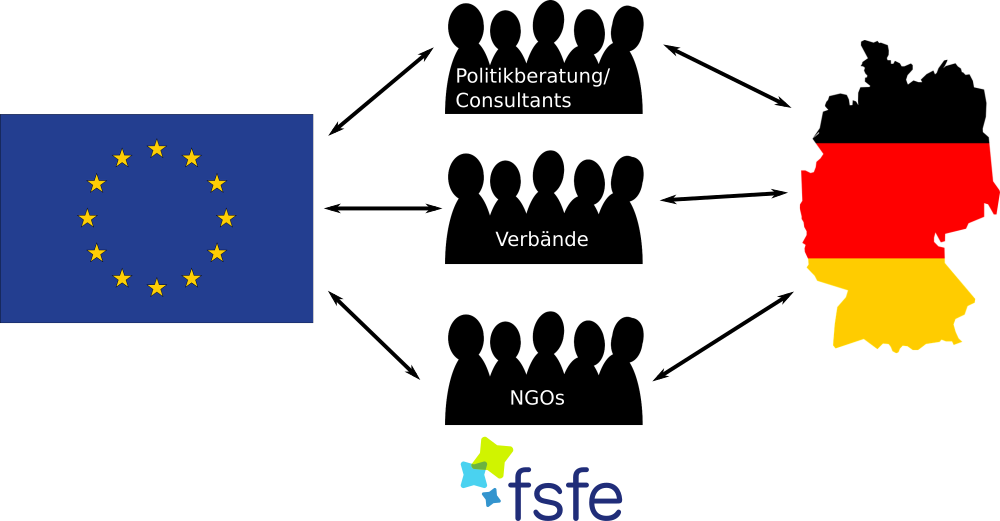
\includegraphics[width=\textwidth]{struktur}
	\centering
	\caption{Struktur des Lobbyismus}
	\label{fig:structure_image}
\end{figure}
In unserer heutigen Informationsgesellschaft ist klar zu verzeichnen, dass sich
die allgemeine Komplexität der Aufgaben, denen ein Staat, dessen Regierung und 
Bürger gegenüber stehen immens gestiegen ist und weiter wachsen wird.
Daraus entstehen folglich Probleme in der Entscheidungsfindung über Gesetze, da 
um solche durchschauen und verstehen zu können eine hohe Menge an Fachwissen 
nötig ist, die sich unmöglich eine einzelne Person aneignen kann. An der 
Schnittstelle, an welcher genau dieses Wissen der Exekutive zugeführt wird, 
setzt Interessenvertretung im allgemeinen an. Es wird im Prinzip mit Wissen 
bzw. Information Handel getrieben. Dies ist auch der Grund warum Leif und 
Speth\cite{LeifSpeth200312} Lobbyismus zu einer Branche erheben.

Leif und Speth führen weiterhin die Akteure des Lobbyismus an, unter 
welchen sich PR- und Image-Berater, Vertreter, Verbände, Wirtschaftsgruppen und 
NGOs befinden. Speziell die Verbände werden hier auch wissenschaftlich 
und vor allem im Kontext der Bundesrepublik Deutschland betrachtet.

Folglich wird dann auch auf Unterschiede zwischen Lobbyismus auf nationaler, 
europäischer oder Globaler Ebene geschlossen. Wie auf 
Abb.~\ref{fig:structure_image} 
deutlich wird, können z.B. die selben Lobbyingorganisationen sowohl auf 
Bundesebene als auch auf Europäischer ebene wirken. Allerdings müssen sie 
natürlich mit verschiedenen Regierungsformalismen und Bürokratien interagieren.

\subsection{Probleme}
Zu den geographischen Unterschieden gehört zusätzlich auch die Wahrnehmung bzw. 
Wertung des 
Lobbyismus als Hilfe bis hin zur Korruption. Nach Leif und Speth liegen die 
Gründe hierfür in den unterschiedlichen Ansichtsweisen bezüglich der jeweiligen 
in den Staaten vorherrschenden Demokratiemodelle. Die beiden Autoren führen 
hierbei den Pluralismus als Lobbyismus-akzeptierendes, wenn nicht sogar durch 
den Lobbyismus begründendes Modell an, welches dem Rousseau`schen Modell 
gegenübergestellt wird. Letzteres definiert Grundsätze der direkten Demokratie, 
in welcher es durch das Fehlen von 
''Vertretungskörperschaften``\cite{WikiIdentitaetstheorie} keinen 
Angriffspunkt, an dem Interessenvertretung wirken kann, gibt.

Es gibt allerdings auch modellunabhängige Kritikpunkte. Gesetzt dem Fall, man 
ist in der Lage wissenschaftlich abzuschätzen, wie viele Gesetze durch einwirken
von Interessengruppen und wie viele durch den Wahlprozess verabschiedet werden, 
könnte man zeigen das die Wahlen keinen großen Einfluss mehr auf die 
Entscheidungsfindung haben. Das Modell der Demokratie würde dadurch ad absurdum 
geführt werden. Es soll in dieser Arbeit kein ''Beweis`` für diese Aussage 
erbracht werden. Es ist jedoch davon auszugehen dass sie mittlerweile der 
Wahrheit entspricht.

% transparenzproblem und Asymmetrie der Interessenvertretungskraft
Es stellt sich daraus die Frage, ob Lobbyismus in einem demokratischen Kontext 
existieren kann. Diese kann nur mit ''Ja`` beantwortet werden, wenn alle 
demokratiebedrohenden Faktoren behandelt und formalisiert werden. Das 
Kernproblem des Lobbyismus wurde bereits genannt. Die Interessenvertretung ist 
im Allgemein nicht gesetzlich geregelt, bzw. fehlt es ihr an ausreichend 
Transparenz, um unbürokratisch zu verlaufen. Somit ist folglich nicht 
gewährleistet, 
dass auch Interessengruppen, welche finanziell nicht gut aufgestellt sind, die 
selbe Chance haben, ihre Ziele in den Politikprozess einzubringen. Beispiele 
wären hier Naturschutzvereine oder Menschenrechtsorganisationen, welche 
meistens nur begrenzt durch staatliche Förderungen und Spenden finanziert 
werden und somit nicht die selbe Wirksamkeit erzielen können wie eine 
Organisation, die von einem Großkonzern gefördert wird.

\subsection{Formalisierungsversuche}
% Verhaltenskodex der Europäischen Kommession (Rechtsanwaltskanzleien)
Es existieren bereits Versuche, genau diese Probleme zu lösen. Der ``Rahmen für 
die Beziehungen zu Interessenvertretern''\cite{EuLobbyCodex} ist zum Beispiel 
ein Versuch der 
Europäischen Kommission, die Beeinflussung durch Akteure des Lobbyismus in 
geregelte Bahnen zu lenken. Es wird hier der Aufbau eines freiwilligen 
Registers angegangen, in welches sich Interessenvertreter eintragen können, 
insofern sie die Einhaltung des Codex beachten. Wer den Codex nicht beachtet 
würde öffentlich wieder aus dem Register ausgetragen werden. Somit kann sich 
hier eine Art Whitelist-Prinzip etablieren, in welchem - wenn es genügend 
Registereintragungen gibt - eine Nichteintragung gleichbedeutend mit einer 
schlechten ``Lobbyingbewertung'' wäre. Der Codex selbst regt zur Transparenz 
an, indem er die Offenlegung der Interessen, Klienten und 
Arbeitgeberorganisationen der Interessenvertreter fordert. Allerdings kann 
angenommen werden, dass Aktionen bei Nichteinhaltung des Codex nicht die 
mögliche Bestrafungswirksamkeit ausnutzen, wie folgendes Zitat zeigt:
\begin{displayquote}
``Im Falle eines mutmaßlichen Verstoßes kann jedermann bei der Kommission 
Beschwerde einlegen. Liegt der Kommission eine Beschwerde vor, wird sie vor der 
Einleitung eines förmlichen Verfahrens die betreffende Organisation bzw. 
Einrichtung um Klärung der Angelegenheit bitten und sie auffordern, die Regeln 
einzuhalten und gegebenenfalls falsche oder irreführende Informationen im 
Register zu berichtigen.''\cite{EuLobbyCodex}
\end{displayquote}
Ein weiterer Kritikpunkt an der Formulierung des Codex ist, dass er gezielt 
``Tätigkeiten im Zusammenhang mit Rechtsberatung''\cite{EuLobbyCodex} von der 
Pflicht sich in das Register einzutragen befreit. Diese werden jedoch in 
anderen Werken\cite{LeifSpeth200312} genau als Akteure der politischen 
Einflussnahme angeführt, was eine Art Hintertür bilden könnte.

% SEAP
Die Formalisierung der Aspekte des Lobbyismus geht aber auch von anderen 
Stellen aus. Hier angeführt sei die Society of European Affairs Professionals 
(SEAP), welche eine Organisation darstellt, die Schulungen für angehende 
Lobbyisten zur Verfügung stellt. Der wohl hier wichtigste Fakt ist jedoch, dass 
die Zugangs- bzw. Kontaktnetzwerke, welche die Akteure nutzen können, 
gebündelt und festgehalten werden, was wahrscheinlich effizienteres Lobbying 
ermöglicht. Es gibt noch mehr Organisationen wie die SEAP welche alle ihren 
eigenen Code of Conduct pflegen.\cite{2012lobbyists}

\subsection{Metalobbyismus}
Bei dem hier eingeführten Begriff des Metalobbyismus handelt es sich um ein 
spezielles Problem, was bei der bereits behandelten Schematisierung des 
Lobbyismus eintreten müsste. Dieses zeigt sich genau dann, wenn Unternehmen wie 
die SEAP wieder Interessenvertretung für ihre eigene Branche betreiben und 
genau dann, wenn Lobbyismus eine eigenständige gewinnbringende Sparte im Markt 
bildet. Daraus könnte ein gewisser Selbsterhaltungsmechanismus der 
Lobbyingorganisationen entstehen welcher diesen wiederum zu gute kommt und dazu 
führen könnte dass sich diese Organisationen nach und nach von ihrem 
ursprünglichen Aufgabengebiet ablösen.

Es ist somit ein ausreichender Grundstock an Informationen über das Thema 
Lobbyismus gelegt um im folgenden genau zu klären, inwiefern die FSFE Lobbying 
betreibt.

\newpage
\section{Die FSFE als Lobbyorganisation}
\epigraph{Politischen Wandel und politische Meinungsbildung zugunsten Freier 
Software zu beeinflussen ist sicherlich ein wichtiger Aspekt unserer 
Arbeit}{George Greve~\cite{PLGreveInterView}}
Die Frage ob es sich bei der FSFE um eine Lobbyorganisation handelt ist mit den 
Aussagen von George Greve~\cite{PLGreveInterView} schnell mit ``Ja'' 
beantwortet, was die Betrachtung der Art der politischen Einflussnahme 
wesentlicher in den Fokus rückt. Greve nimmt öffentlich und direkt 
dazu Stellung und führt Beispiele für die Einflussnahme durch die FSFE auf.

% Einordnung
Strukturell ordnet sich die FSFE in die Gruppe der NGOs ein, wodurch sich die 
Schnittstellen des Lobbying auf Öffentlichkeitsarbeit und Teilnahme an 
Kongressen belaufen. Es lassen sich zusätzlich auch Beispiele für indirektes 
Lobbying finden, wie z.B. das Zuarbeiten von Informationen für den 
\emph{Foundation~for~a~Free~Information~Infrastructure~e.V.~(FFII)}~\cite{PLGreveInterView}.
Die in diesem Fall vorliegende Zurückhaltung der Stellungsnahme über 
Softwarepatente, lässt hier auch ein hohes Maß an Taktik vermuten.

% Finanzielle Einordnung
Um die Arbeit der FSFE auf dem globalen Maß zu gewährleisten ist ein 
entsprechendes Budget nötigt. Wie auf Abb.~\ref{fig:finances_image} deutlich 
wird, ist Dieses in den vergangenen Jahren reichhaltig angestiegen. Während 
Greve 
im Jahr 2004 noch von einem Budget von 60.000 \euro sprach, waren es im Jahr 
2013 fast 400.000 \euro. Dies entspricht ungefähr dem Lobbybudget von Microsoft 
2004, welches sich damals auf rund 300.000 \$ belief.\cite{PLGreveInterView}
\begin{figure}[h]
    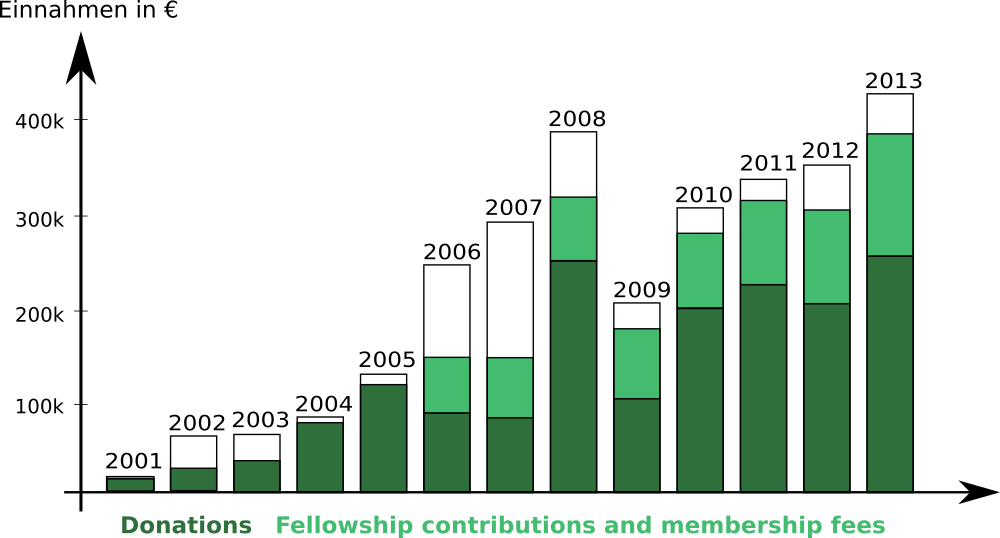
\includegraphics[width=\textwidth]{finanzen1}
    \centering
    \caption{Budgetverlauf der FSFE}
    \label{fig:finances_image}
\end{figure}
Abbildung~\ref{fig:finances_image} zeigt, dass der Großteil des Einkommens der 
FSFE durch Spenden von Unternehmen kommt, wobei mehrere Marktgrößen wie Google, 
HP und Intel darunter aufgeführt sind. Hier tut sich eine Schnittstelle für 
indirekten Lobbyismus auf, welche nur durch Transparenz vertrauenswürdig 
gemacht werden kann. Natürlich ist es hier nicht möglich zu ermitteln, ob und 
wie es Absprachen ``hinter den Kulissen'' zwischen der FSFE und den 
aufgeführten Unternehmen gab. Jedoch weiß man z.B. von Google, dass sie seit 
jeher 
eine mehrseitige Förderungspolitik durchführen, wie man beispielsweise an den 
Projekten \emph{Chromium} und \emph{Chrome} sieht, wobei Chromium den zumindest 
teilweise Free-Software-konformen Teil übernimmt und dann mit diversen 
proprietären 
\emph{Privacy~Extensions} als \emph{Google~Chrome} ausgeliefert wird. In 
anderen Bereichen 
gibt sich die FSFE sehr transparent. Alle Mitglieder sind 
gelistet und auch die Informationen über jeweilige Kampagnen sind sehr 
ausführlich. Auch der innere Entscheidungsprozess findet nach Greves 
\cite{PLGreveInterView} demokratisch mittels eines Konsensprinzips statt, 
welches sich aber in Notfällen durch ein Mehrheitsprinzip überstimmen lässt.

\subsection{Wirken der FSFE}
Der Wirkungsbereich der FSFE skaliert konträr zum Name auf globale Reichweite. 
Dies zeigt unter anderem die Teilnahme am 
\emph{World~Summit~on~the~Information~Society~(WSIS)}. In dessen 
Commitment~\cite{WSISTunisCommitment} werden klar Zugeständnisse gegenüber 
Freier Software gemacht, indem Free Software als gleichwertiger Partner 
gegenüber proprietärer Software angebracht wird. Die Wirkung solcher Versprechen
ist jedoch nicht wirklich absehbar, kann aber durchaus die Entwicklung von 
Trends bewirken und die durchschnittliche Auffassung über solche Themen 
beeinflussen.

% Kartellklage gegen Microsoft
Etwas klarer waren die Auswirkungen im Jahr 2001, als die FSFE die 
\emph{Generaldirektion~Wettbewerb} der Europäischen Kommission bezüglich einer 
Kartellklage gegen Microsoft beriet. Zusätzlich fand Kommunikation mit den 
Entwicklern des ``Samba''-Projektes statt, welche sich an der Geschlossenheit 
der Protokolle, die Microsoft benutzt, um die Windows-eigenen 
Networksharing-Dienste zu implementieren, störten. Es wird dabei angemahnt, 
dass durch die Nichtverfügbarkeit der Spezifikation dieser Protokolle andere 
Unternehmen bzw. Projekte wie z.B. Samba nicht in der Lage sind, in Wettbewerb 
mit Microsoft zu treten, da sie keine kompatiblen Implementation realisieren 
können. Microsoft verstößt mit dieser Strategie gegen gängige Designpattern, da 
eine Aufgabe von Protokollen genau die Interoperabilität ist. Folgende Aussage 
der FSFE trifft den Sachverhalt sehr präzise auf den Punkt. ``Die 
Information, die Microsoft hatte, war nicht geheim, weil sie wertvoll war, sie 
war nur wertvoll, weil sie geheim war.'' \cite{FsfeEUvsMS} Es handelt sich 
dabei um eine übliche Marktstrategie, welche allerdings hier offensichtlich den 
technologischen Fortschritt behindert.

% Secureboot (FSFE website)
Eine ähnliche Thematik, welche allerdings noch nicht soweit fortgeschritten 
ist, stellt \emph{Secure~Boot} dar. Diese Technologie ist dafür verantwortlich, 
dass z.B. der Bootloader eines Systems nur dann ausgeführt wird, wenn es sich 
dabei um eine signierte Software handelt und diese Signatur auch vom 
Gerätehersteller vorinstalliert wurde. Das ermöglicht selbigem, ein 
Installieren von Bootloadern wie \emph{Grub} oder \emph{Gummiboot} zu 
unterbinden. Das Ziel der Sicherheit geht hier deutlich mit einer Einschränkung 
der vom Nutzer ausgehenden Kontrolle einher. Der von Leif und Speth erwähnte 
``Mantel des Gemeinwohls'' \cite{LeifSpeth200312} könnte hier durchaus der 
Vater des Gedankens sein. Die FSFE fordert hier ein eindeutiges Kennzeichnen 
von Geräten, dessen Benutzung in geschilderter Weiße eingeschränkt ist. 
\cite{FsfeSecureBoot} Das Thema Sicherheit besitzt allerdings im Allgemeinen 
Eigenschaften, die es für gezielte Einflussnahme empfänglich machen. So muss 
z.B. Signierung von einer zentralen Instanz ausgehen die bestimmt was 
vertrauenswürdig ist und was nicht. Diese Instanz kann allerdings selber nie 
als vertrauenswürdig gelten, da sie immer von außen und auch intransparent 
beeinflussbar ist. Des weiteren handelt es sich bei Verfahren zur 
Gewährleistung von Sicherheit nach Definition immer um eine 
Kontrolleinschränkung, was offensichtlich der Nutzungsfreiheit widerspricht. 
Dies soll allerdings nicht zwangsweise bedeuten, dass es nicht möglich ist, 
einen konstruktiven und verträglichen Mittelweg zwischen Sicherheit und 
Nutzerfreiheit zu finden.

\section{Unterschied zu anderen Lobbyingarten}
Um nun das Lobbying der FSFE in einen angemessenen Kontext zu setzen, ist es 
nötig Lobbystrukturen anderer Themenbereiche mit in die Arbeit einzubeziehen. 
Es 
wird sich dabei herausstellen, dass es fundamentale Unterschiede in Intensität 
und Finanzlage gibt, aber auch Gemeinsamkeiten in der Struktur existieren.
\subsection{Agrarlobbyismus}
Die hier fokussierte Gegenüberstellung soll sich mit dem Lobbyismus im 
Agrarsektor 
beschäftigen. Dieser weißt natürlich eine wesentlich längere Entwicklungsphase 
auf als der IT-Sektor und die pure Notwendigkeit dieser Branche hat 
weitreichende Auswirkung in der Finanzierung wie z.B. Subventionen. Weiterhin 
wird dadurch auch die Verteilung der Interessengruppen maßgeblich beeinflusst.

% Entwicklung des Marktes
Neimann \cite{Neimann200312} schildert die Entwicklung des Agrar-Marktes vom 
zweiten Weltkrieg bis 
heute, woraus essentielle Erkenntnisse hervorgehen, die zur Ableitung der 
Struktur des Agrarlobbyismus wichtig sind. Dabei wird allerdings vorerst nur 
Deutschland betrachtet, dessen Entwicklung als repräsentativ gelten soll. So 
wird der Bereich kurz nach dem Weltkrieg als sehr lukrativ geschildert, wobei 
der Agrar-Markt größtenteils von Kleinbauern dominiert wurde. Diese enorm 
heterogene Masse an Erzeugern stellt sehr schwierige Anforderungen an den 
Aufbau einer wirklich repräsentativen Interessenvertretung.

% DBV
Ob der bereits 1948 gegründete \emph{Deutsche Bauernverband (DBV)} genau diese 
Anforderungen erfüllt, wird 
kontrovers diskutiert. \cite{Neimann200312} Dies liegt unter anderem am 
Strukturwandel des so genannten \emph{Agrobusiness}. So wurden bis heute die 
Kleinbauern, welche größtenteils klassische und umweltverträglichere Methodiken 
zum Anbau oder Viehzucht verwenden, von immer größer werdenden Konzernen 
verdrängt. Dies lag zum Teil daran, dass die Nahrungsmittelproduktion 
effizienter werden musste, da die Weltmarktpreise eher niedriger als die 
Eigenproduktionspreise waren. Ein weiterer Grund könnte in der schieren Größe 
der durch den DBV zu bündelnden Interessen liegen, da es sich um einen 
Dachverband handelt, welcher 18 untergeordnete Landesverbände mit insgesamt 
430.000 Mitgliedern besitzt. \cite{Neimann200312} Es wird also deutlich, dass 
es sehr starke 
Unterschiede zum wirtschaftlichen Raum der FSFE gibt.

Die jedoch wohl größten Differenzen findet man im Thema Transparenz und der 
damit verbunden Professionalisierung. Während die FSFE genau Finanzen und 
Mitgliederwerdegänge offen stellt, passiert dies beim DBV eher zäh auf 
Nachfrage. Dies könnte z.B. an der Legitimierung der Interessenvertretung 
liegen. Die FSFE muss sich schließlich, um wirklich Einfluss auf die Politik zu 
üben, eine gewisse Glaubwürdigkeit und Popularität verschaffen um gehört zu 
werden. Es könnte somit ein Konkurrenzkampf zwischen verschiedenen NGOs 
entstehen welcher um den meisten Einfluss ringt. Konträr dagegen steht der DVB 
nahezu in einer Monopolposition bezüglich Interessenvertretung. So wird er von 
Neimann sogar als ``Halbstaatlicher Dienstleister mit Vertretungsmonopol'' 
\cite{Neimann200312} bezeichnet. Außerdem wird angemahnt, dass in der 
Hierarchiekette der Bauernverbände auf Ebene der Landesverbände das 
Nach-Oben-Streben diverser Alternativverbände verhindert wird und somit die 
Repräsentativität der Interessen verloren geht.

% Subventionen
Ein weiterer wichtiger Punkt welcher im Lobbysektor der FSFE eine nicht so 
große Rolle spielt, ist die Verteilung von Subventionen. Diese ist 
allerdings in der Agrarbranche von großer Wichtigkeit, da die Weltmarktpreise 
für die 
Erzeugnisse sehr unterschiedlich sind und dadurch z.B. die EU-Kommission 
Subventionen an die Mitgliedsstaaten vergibt. So betrugen die Hilfen im Jahr 
2010 ca. 57,1 Milliarden Euro, was nahezu die Hälfte des kompletten 
EU-Haushaltes ausmacht. \cite{ZeitEuroAgrar} Hier wird auch angemahnt, dass die 
Aufteilung der Mittel auf die Mitgliedsstaaten sehr ungleichmäßig war
und innerhalb der Länder auch zum Großteil in Großkonzerne und nicht in die 
Förderung von Kleinbauern floss. \cite{ZeitEuroAgrar}

%
Es wird auch deutlich, dass sowohl der DVB als auch die FSFE auf Europaebene 
agieren. So war z.B. Gerd Sonnenleiter Präsident des DVB auch bis heute 
Präsident des \emph{Comité des organisations professionnelles agricoles 
(COPA)}. \cite{WikiCopa}

% Monsanto
Ob sich der Einflussbereich wie der der FSFE auch weltweit ausbreitet ist 
fraglich. 
Allerdings 
gibt es durchaus Lobbyismus-betreibende Unternehmen, welche auf globaler Ebene 
wirken. Als extremstes Beispiel sei hier der US-Konzern \emph{Monsanto} 
angeführt, dessen Lobbyingintesität sicherlich weltweit seines Gleichen sucht. 
Die pure Aggressivität auf dem Markt steht dem in Nichts nach. So gibt es sogar 
ein Zusammenschluss aus mehreren Organisationen, die das Unternehmen im Jahr 
2016 vor den Europäischen Gerichtshof in Den Haag, wegen Verbrechen gegen die 
Menschheit und \emph{Ökozid} bringen wollen. \cite{MonsantoTrail}

Im Gegensatz zum DVB oder der FSFE, betreibt Monsanto höchstwahrscheinlich 
direktes Lobbying über US-Botschafter \cite{WikiMonsanto} und greift so direkt 
in die Politik ein. Die Kette der Anschuldigungen reicht von 
Förderung zweifelhafter wissenschaftlicher Veröffentlichungen bis hin zur 
Denunzierung 
von Wissenschaftlern, welche die Umweltunverträglichkeit der von Monsanto 
vertriebenen Pestizide, kritisieren.

\subsection{Fazit}
Es ist also deutlich erkennbar, dass die FSFE als bekennende Lobbyorganisation 
einen anderen, transparenteren Weg verfolgt und demokratischer ist als seine 
Mitstreiter. Vielleicht liegt dies unter anderem daran, dass sich die 
Menschen, 
welche sich im Umfeld der FSFE formieren, durch die Gedanken über Freie 
Software, in einem freieren und durchsichtigeren Kulturfeld befinden als die 
nicht vertretenen Kleinbauern oder die aggressiven Vorstände des Konzerns 
Monsanto. 
% TODO rephrase maybe

\section{Schluss}
Die Arbeit hat wie angekündigt gezeigt, dass der intuitive Lobbyismusvorwurf 
sehr relativiert werden kann, da schon allein der Bergriff als solches positive 
als auch negative Ausprägungen besitzt. Die ausgiebige Komplexität, welche in 
der Struktur der verschiedenen Lobbyismusvorkommen steckt, macht deutlich, dass 
es nötig ist die einzelnen Themengebiete getrennt zu behandeln, um die 
jeweilige 
vorherrschende Transparenz verbessern zu können. Es wird deutlich, dass gerade 
diese 
Transparenz der Kernfaktor sein könnte, um ein Qualitätsmaß für lobbyistische 
Tätigkeiten zu bilden.

Dafür, dass man um eine Professionalisierung bzw. Formalisierung nicht mehr 
herum kommt, gibt es mehrere Gründe. Zum einen die immer größer werdende 
Spezialisierung der Themengebiete, welche Politik und Gesellschaft betreffen. 
Zum anderen stellt Lobbyismus in seinem Grundsatz einen völlig natürlichen Weg
Ziele zu verwirklichen dar. Der allerdings wichtigste Grund ist die 
Verbesserung 
der Transparenz und die damit verbundene Möglichkeit für Interessengruppen 
wieder wirklich repräsentativ vertreten zu werden.

Es wurden bereits Maßnahmen zur Realisierung des Geforderten aufgenommen, wie 
z.B. der Code Of Conduct der EU-Kommission \cite{EuLobbyCodex}. Ob solche eher 
freiwilligen Regulierungsversuche von Nutzen sind, ist fraglich, schaffen sie 
jedoch einen Anfang, auf welchem aufgebaut werden kann.

Eine weiterer Vorschlag wäre z.B. die Überarbeitung des jetzigen deutschen 
Parteisystems hin zu einer Menge von verschiedenen themenbezogenen Pools von 
Parteien. So könnte es Verschiedene Pools für z.B. IT, Gesundheitswesen, 
Wirtschaft usw. geben in denen mehrere Parteien konkurrieren. Durch die hier 
gegebene Struktur wäre es wieder möglich, dass die Parteien sich mit 
ausreichend Wissen über ihr Themengebiet ausstatten könnten und vor allen 
Dingen, dass der Wähler in dem Themenpool wählen kann in dem er sich am besten 
auskennt, was die Wirksamkeit von demokratischen Wahlen wieder erhöhen würde.

Allerdings muss beachtet werden, dass solche weitreichenden Änderungen kaum 
möglich sind, da nach der These des Metalobbyismus die lobbyistischen 
Strukturen sich selbst erhalten und diesem Umschwung entgegen wirken würden. 
Dies wird das zentrale Problem in der Antwort der folgenden Frage sein.
Wie erreichen wir wieder eine wirkliche Demokratie an dessen 
Entscheidungsfindung sich jeder Wahlberechtigte effektiv beteiligen kann, und 
wichtiger, ist das sinnvoll?

\newpage
\printbibliography

\end{document}
